\documentclass[sigconf,nonacm]{acmart}

% Remove ACM-specific elements for preprint
\settopmatter{printacmref=false}
\renewcommand\footnotetextcopyrightpermission[1]{}
\pagestyle{plain}

\usepackage{lmodern}
\usepackage{booktabs}
\usepackage{listings}
\usepackage{xcolor}
\usepackage{amsmath,amssymb}
\usepackage{subcaption}
\usepackage{balance}
\usepackage{xspace}
\usepackage{multirow}

% Code listing style
\lstset{
  basicstyle=\ttfamily\small,
  keywordstyle=\color{blue}\bfseries,
  commentstyle=\color{gray},
  stringstyle=\color{red},
  numbers=left,
  numberstyle=\tiny\color{gray},
  breaklines=true,
  frame=single,
  language=C,
  captionpos=b
}

\newcommand{\sys}{\textsc{Sage}\xspace}
\newcommand{\ie}{\textit{i.e.}\xspace}
\newcommand{\eg}{\textit{e.g.}\xspace}
\newcommand{\etal}{\textit{et~al.}\xspace}

\begin{document}

\title{\sys: Zero-Multiply Neural Network Inference in eBPF/XDP \\via Operator Co-Design and Quantization-Aware Training}

\author{Anonymous}
\affiliation{%
  \institution{Anonymous Institution}
  \country{}
}
\email{anon@example.com}

\begin{abstract}
Deploying neural networks inside the Linux kernel via eBPF/XDP enables
microsecond-level network intrusion detection, but the eBPF execution
environment imposes severe constraints: no floating point, a 512-byte
stack, and limited instruction budgets.
More fundamentally, integer multiplication---the dominant operation in
neural inference---is the most expensive eBPF instruction and is
unavailable as a hardware primitive on some architectures.

We present \sys (\textbf{S}afe \textbf{A}daptive In-Kernel Neural
Inference En\textbf{g}in\textbf{e}), the first eBPF/XDP neural network
that achieves \emph{zero} multiply instructions.
\sys makes four contributions:
(1)~an int32 fixed-point baseline that \emph{losslessly} preserves float
accuracy (97.64\%);
(2)~\textbf{MapLUT}, which replaces the input layer with BPF-map-based
lookup tables, enabling runtime model hot-updates;
(3)~\textbf{Quantization-Aware Training (QAT) with Straight-Through
Estimation}, which makes ternary weight quantization viable for severely
imbalanced security data by preserving minority-class gradients during
training; and
(4)~\textbf{MapLUT + Ternary-QAT}, the first \emph{fully zero-multiply}
neural network in eBPF, achieving 95.78\% accuracy (512 bins) with 1,424
BPF instructions---\emph{none} of which are multiplications.
Notably, PortScan F1 \emph{improves} from 0.597 (float baseline) to
0.629 under MapLUT + Ternary-QAT, because QAT with focal loss forces
the model to focus on hard, rare cases.
\end{abstract}

\begin{CCSXML}
<ccs2012>
<concept>
<concept_id>10003033.10003083.10003095</concept_id>
<concept_desc>Networks~Network monitoring</concept_desc>
<concept_significance>500</concept_significance>
</concept>
<concept>
<concept_id>10002978.10003029.10011703</concept_id>
<concept_desc>Security and privacy~Intrusion detection systems</concept_desc>
<concept_significance>500</concept_significance>
</concept>
</ccs2012>
\end{CCSXML}

\ccsdesc[500]{Networks~Network monitoring}
\ccsdesc[500]{Security and privacy~Intrusion detection systems}

\keywords{eBPF, XDP, zero-multiply inference, quantization-aware training, lookup-table neural network, intrusion detection}

\maketitle

%% ============================================================
\section{Introduction}\label{sec:intro}

Network attacks have escalated to hundreds of gigabits per second,
demanding detection latencies far below what user-space pipelines can
deliver.
The eBPF/XDP subsystem in the Linux kernel offers a compelling
alternative: programs attached at the XDP hook process packets before
they enter the network stack, achieving single-digit microsecond
latency~\cite{zhang2024dsn}.

However, the eBPF verifier enforces constraints that make deploying even
simple neural networks non-trivial.
Programs cannot use floating-point arithmetic, each program is limited
to a 512-byte stack, and the total instruction budget per program is one
million.
More critically, \emph{integer multiplication is the most expensive eBPF
instruction} and is entirely absent on some architectures (\eg 32-bit
ARM), where it must be emulated in software.
Prior in-kernel neural networks~\cite{zhang2024dsn,hara2023nn} rely
heavily on multiply instructions for matrix--vector products,
which dominate both instruction count and latency.

Our key insight is that \emph{zero-multiply neural inference is
achievable through operator co-design}, but naively applying ternary
weight quantization to models trained on imbalanced security data causes
catastrophic minority-class collapse.
We show that Quantization-Aware Training (QAT) with the
Straight-Through Estimator (STE)~\cite{bengio2013ste} resolves this
problem, and when combined with lookup-table-based input layers, yields
the \emph{first fully zero-multiply neural network in eBPF/XDP}.

\sys makes four contributions:

\begin{enumerate}
\item \textbf{Int32 fixed-point inference} (\S\ref{sec:background}).
The enlargement method~\cite{zhang2024dsn} with scale $s = 2^{16}$
achieves \emph{lossless} quantization: 97.64\% accuracy, identical to
the float baseline on CIC-IDS-2017.

\item \textbf{MapLUT} (\S\ref{sec:maplut}).
The input layer's matrix multiplication is replaced by a BPF
\texttt{PERCPU\_ARRAY} map storing precomputed partial sums.
Because the LUT resides in a BPF map, model weights can be hot-updated
at runtime via \texttt{bpf\_map\_update\_elem()} with zero downtime---a
unique advantage over compiled-in weights.

\item \textbf{QAT with STE for ternary quantization}
(\S\ref{sec:qat}).
Post-hoc ternary quantization of the original float-trained model
destroys minority-class performance (PortScan F1 drops from 0.597 to
0.020).
Our two-phase QAT procedure---float warmup followed by STE-based ternary
training with focal loss~\cite{lin2017focal}---recovers minority classes
and \emph{exceeds} the float baseline's PortScan F1.

\item \textbf{MapLUT + Ternary-QAT = zero-multiply NN}
(\S\ref{sec:eval}).
The full pipeline achieves 95.78\% accuracy (512 bins) with 1,424 BPF
instructions, zero of which are multiplications.
PortScan F1 improves from 0.597 (float) to 0.629.
\end{enumerate}

Table~\ref{tab:headline} summarizes the instruction-level result: \sys
V3 is the \emph{first zero-multiply neural network inference engine in
eBPF/XDP}.

\begin{table}[t]
\centering
\caption{BPF instruction profile across \sys versions.
Multiply counts verified by \texttt{llvm-objdump~|~grep~mul}.}
\label{tab:headline}
\small
\begin{tabular}{lcc}
\toprule
Version & Total Insns & Multiply Insns \\
\midrule
V0-Baseline (int32 matmul)           & 804    & 15 \\
V2-Fused+Ternary+Exit               & 1{,}437 & 16 \\
\textbf{V3-MapLUT+Ternary+Exit}     & \textbf{1{,}424} & \textbf{0} \\
V3b-MapLUT+Int32                     & 1{,}016 & 5 \\
\bottomrule
\end{tabular}
\end{table}


%% ============================================================
\section{Background}\label{sec:background}

\subsection{eBPF/XDP Constraints}

Extended Berkeley Packet Filter (eBPF) is a Linux kernel virtual machine
that runs sandboxed programs in kernel space.
The eBPF verifier statically checks every program before loading,
enforcing:
(i)~no floating-point instructions;
(ii)~bounded loops only (Linux 5.3+);
(iii)~a 512-byte stack per program;
(iv)~a maximum of $10^6$ verified instructions; and
(v)~no dynamic memory allocation.
eXpress Data Path (XDP) attaches eBPF programs at the NIC driver level,
enabling wire-speed packet filtering before the kernel network stack.

\textbf{Tail calls} allow one eBPF program to transfer control to
another without returning, effectively chaining programs while granting
each its own 512-byte stack frame (maximum chain depth: 33).
\textbf{BPF maps} are kernel-managed key--value stores shared between
eBPF programs and user space.
Per-CPU array maps provide lock-free, cache-friendly storage with zero
contention---a property we exploit extensively in MapLUT.

\subsection{Enlargement-Method Quantization}

The enlargement method~\cite{zhang2024dsn} converts a floating-point MLP
to integer-only inference.
Given a scale factor $s = 2^b$, weights are quantized as
$W_E = \text{round}(s \cdot W)$ and biases as
$B_E = \text{round}(s \cdot B)$, both stored as \texttt{int32}.
For each layer, inference computes:
\begin{equation}\label{eq:enlarge}
z_i = \Bigl(\sum_{j} W_E[i][j] \cdot x[j]\Bigr) \gg b \;+\; B_E[i]
\end{equation}
The accumulation uses \texttt{int64} to avoid intermediate overflow, and
the final argmax is scale-invariant.
On our CIC-IDS-2017 task, this method achieves \emph{lossless}
quantization: 97.64\% accuracy, identical to the float baseline
(Table~\ref{tab:ablation}).
This forms the \emph{baseline}; \sys replaces the per-layer multiply
operations in Eq.~\eqref{eq:enlarge} with multiply-free alternatives.

\subsection{Prior eBPF ML Work}

Bachl~\etal~\cite{bachl2021dt} deployed decision trees in eBPF for
CIC-IDS-2017 classification, achieving ${\sim}$99\% binary accuracy but
with $>$32\,KB memory.
Hara~\etal~\cite{hara2023nn} demonstrated int8 NN inference in eBPF
with 84\% latency reduction over user space, but with significant accuracy
loss.
Zhang~\etal~\cite{zhang2024dsn} introduced the enlargement method with
tail-call chains, the closest work to ours but limited to binary
classification and reliant on multiply instructions.
None of these systems have pursued multiply-free inference.


%% ============================================================
\section{System Design}\label{sec:design}

\sys uses a 4-class MLP with architecture $[12, 64, 64, 4]$:
12 flow features extracted from packet headers, two 64-unit hidden
layers with ReLU, and a 4-class output.
Two distinct training procedures produce two models, each serving a
specific role in the evaluation:
\begin{itemize}
\item \textbf{Original model}: trained with standard cross-entropy loss.
Used for the Float and Int32 baselines.
\item \textbf{QAT model}: trained with the two-phase QAT procedure
described in \S\ref{sec:qat}.
Used for all Ternary-QAT and MapLUT+Ternary-QAT configurations.
\end{itemize}
All reported numbers clearly indicate which model produced them.
Figure~\ref{fig:instructions} shows the instruction-level impact of
each operator.

\begin{figure}[t]
\centering
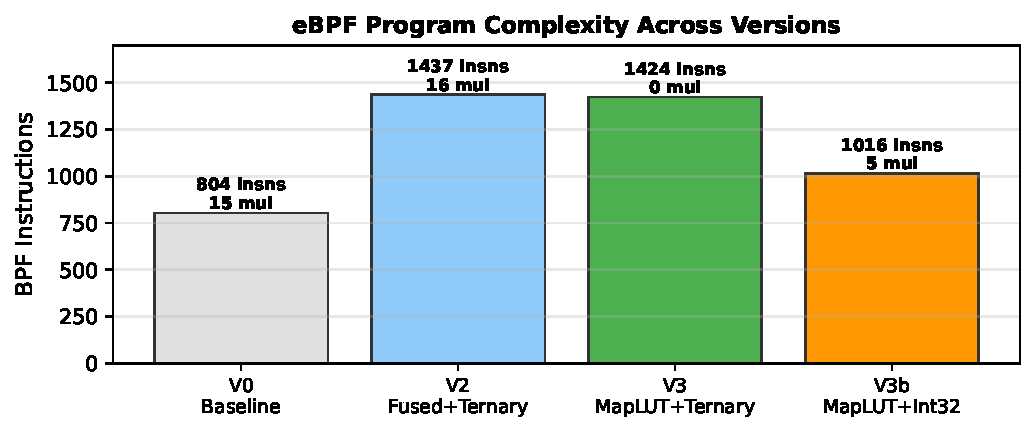
\includegraphics[width=\columnwidth]{figures/instruction_comparison.pdf}
\caption{BPF instruction breakdown.
V3 (MapLUT+TernaryShift) achieves zero multiply instructions.
V3b (MapLUT+Int32) retains 5 multiplies in hidden layers.}
\label{fig:instructions}
\end{figure}

\subsection{MapLUT: Lookup-Table Input Layer}\label{sec:maplut}

\textbf{Problem.}
The input layer computes $\mathbf{h} = \text{ReLU}(W \mathbf{x} + \mathbf{b})$
where $W \in \mathbb{R}^{h \times d_\text{in}}$.
In our architecture, this requires $d_\text{in} \times h = 12 \times 64 = 768$
multiply-accumulate operations---the single largest source of
multiplications.

\textbf{Insight.}
Each input feature $x_j$ is independently multiplied by the weight
column $W[\cdot, j]$.
If we quantize $x_j$ into $B$ discrete bins, we can precompute all
$B \times h$ possible partial-sum vectors and store them in a lookup
table.
At inference time, a single table lookup replaces $h$ multiplications.

\textbf{Bin quantization.}
Each feature $j$ is quantized to a bin index:
\begin{equation}\label{eq:bin}
\text{bin}_j = \text{clamp}\!\bigl(\,(x_j - \text{offset}_j) \gg \text{shift}_j,\; 0,\; B{-}1\bigr)
\end{equation}
The offset and shift parameters are calibrated from training data
statistics.
Crucially, Eq.~\eqref{eq:bin} uses only subtraction and bit shift---no
multiplication.

\textbf{LUT construction.}
For each feature $j$, bin $b$, and hidden unit $i$:
\begin{equation}\label{eq:lut}
\text{LUT}[j, b, i] = \text{round}\!\bigl(W[i,j] \cdot \text{center}(j, b) \cdot s\bigr)
\end{equation}
where $\text{center}(j,b)$ is the representative value of bin $b$ for
feature $j$, and $s = 2^{16}$ is the quantization scale.
The LUT is computed offline and loaded into a BPF \texttt{PERCPU\_ARRAY}
map.

\textbf{Inference.}
The forward pass for layer~0 becomes:
\begin{equation}
\text{hidden}[i] \mathrel{+}= \text{LUT}[j, \text{bin}_j, i] \quad \forall\, j \in [0, d_\text{in})
\end{equation}
This is pure addition over $d_\text{in}$ looked-up values per hidden
unit---zero multiplications.

\textbf{Hot-update advantage.}
Because the LUT resides in a BPF map rather than being compiled into
the program text, model updates require only
\texttt{bpf\_map\_update\_elem()} calls from user space---no program
reload, no XDP detach/attach, and zero downtime.
This enables a future online-learning workflow: retrain the model,
recompute the LUT, and push updates to the running datapath atomically.
No prior in-kernel ML system offers this capability.

\subsection{TernaryShift: Multiply-Free Hidden Layers}\label{sec:ternary}

\textbf{Problem.}
Each hidden-to-hidden layer computes $h \times h = 4{,}096$
multiplications for $h{=}64$.

\textbf{Approach.}
We quantize each weight to one of three values
$\{-\alpha, 0, +\alpha\}$ and represent the ternary code in 2 bits:
\texttt{00}$=0$, \texttt{01}$=+\alpha$, \texttt{10}$=-\alpha$.
Sixteen weights are packed into a single \texttt{uint32}.
The scaling factor $\alpha$ is calibrated as
$\alpha = \text{mean}(|w| \mid w \neq 0)$ over the trained weights, and
$\text{alpha\_shift} = \text{round}(16 + \log_2 \alpha)$ converts the
final accumulator to the correct scale via a single left shift.

\textbf{Dot product.}
Listing~\ref{lst:ternary} shows the core ternary dot-product loop.
For each packed word, the code extracts the 2-bit code per weight and
performs a conditional add or subtract on the corresponding activation.
After scanning all words, a single left shift by \texttt{alpha\_shift}
replaces the multiplication by $\alpha$.

\begin{lstlisting}[caption={Ternary dot product (simplified).},label={lst:ternary},float=t]
static __always_inline int32_t
ternary_dot(int32_t *x, uint32_t *packed,
            int n, int alpha_shift) {
  int64_t acc = 0;
  for (int w = 0; w < n/16; w++) {
    uint32_t word = packed[w];
    for (int k = 0; k < 16; k++) {
      uint32_t code = (word >> (k*2)) & 0x3;
      if (code == 1)
        acc += x[w*16 + k];   // +alpha
      else if (code == 2)
        acc -= x[w*16 + k];   // -alpha
      // code==0: skip (zero weight)
    }
  }
  return (int32_t)(acc >> alpha_shift);
}
\end{lstlisting}

\textbf{Result.}
Each hidden layer uses zero multiply instructions.
The packed representation compresses the weight matrix from
$h \times h \times 4 = 16$\,KB to $h \times h / 16 \times 4 = 1$\,KB
for $h{=}64$.
Combined with biases, the full model (ternary layers + biases) fits in
1.8\,KB.

\subsection{Quantization-Aware Training}\label{sec:qat}

\textbf{The problem with post-hoc ternary quantization.}
Applying ternary quantization to weights trained with standard
cross-entropy produces catastrophic results on minority classes.
On CIC-IDS-2017, PortScan (0.08\% of test data) and BruteForce (0.55\%)
rely on precise weight values to distinguish rare attack patterns from
the overwhelming benign majority.
Post-hoc ternarization of the original float model drops PortScan~F1
from 0.597 to 0.020 and BruteForce~F1 from 0.552 to 0.039
(Table~\ref{tab:ablation}).
The original model's weights are optimized for \emph{continuous}
arithmetic; coarsely discretizing them loses the fine-grained
distinctions needed for rare classes.

\textbf{Two-phase QAT with STE.}
We train a \emph{separate} model specifically for ternary deployment
using a two-phase procedure:

\emph{Phase~1: Float warmup} (30 epochs).
The model is trained with focal loss~\cite{lin2017focal} ($\gamma = 3.0$)
and class-balanced oversampling (100K samples per class) to establish
strong minority-class features.
Batch size is 256; learning rate is 0.01.

\emph{Phase~2: QAT with STE} (90 epochs).
Each forward pass quantizes all hidden-layer weights to ternary values
$\{-\alpha, 0, +\alpha\}$ using a threshold $\delta = 0.7 \times
\text{mean}(|W|)$:
\begin{equation}\label{eq:ternary}
\hat{w}_{ij} = \begin{cases}
+\alpha & \text{if } w_{ij} > \delta \\
-\alpha & \text{if } w_{ij} < -\delta \\
0 & \text{otherwise}
\end{cases}
\end{equation}
The forward pass uses $\hat{W}$ (ternary), but the backward pass
computes gradients with respect to the \emph{float shadow
weights}~$W$ via the Straight-Through Estimator
(STE)~\cite{bengio2013ste,jacob2018quant}:
\begin{equation}\label{eq:ste}
\frac{\partial \mathcal{L}}{\partial W} \approx
\frac{\partial \mathcal{L}}{\partial \hat{W}}
\end{equation}
This allows the optimizer to continue updating the continuous weight
parameters, while the model learns representations that are robust to
the ternary discretization at inference time.
Weight clipping at $|W| > 2.0$ prevents gradient explosion during QAT.

\textbf{Why QAT helps minority classes.}
The key mechanism is that STE allows gradients from minority-class
misclassifications to flow back through the ternary quantization
boundary.
During QAT, the model \emph{jointly} optimizes (a)~which weights to
keep nonzero and (b)~the magnitude~$\alpha$, such that the ternary
weight assignment maximally preserves classification power for
\emph{all} classes.
Focal loss ($\gamma = 3.0$) further amplifies the gradient contribution
of hard examples, which are disproportionately from minority classes.
The result is that the QAT model's ternary weights are specifically
structured to handle the imbalanced CIC-IDS-2017 distribution.

\textbf{Important note.}
The QAT model is optimized \emph{exclusively} for ternary inference.
Its float shadow weights are not meaningful as a standalone
classifier (${\sim}$35\% accuracy), because the training objective
drives weights toward ternary-friendly configurations rather than
continuous optima.
All QAT results in this paper use ternary-quantized weights from the
QAT model; all float/int32 results use the separately trained original
model.

\subsection{EarlyExit}\label{sec:earlyexit}

We briefly note that \sys also includes an experimental
confidence-gated EarlyExit mechanism: a lightweight exit head after
Layer~0 that skips remaining tail-call stages when the top-2 logit
margin exceeds a threshold.
In the current design, EarlyExit drops accuracy to 74.88\% when combined
with MapLUT, because the exit head operates on coarsely quantized LUT
features and compounds the discretization error for difficult samples.
We consider EarlyExit a \emph{limitation} of the current system and
leave its improvement to future work; all main results in this paper
are reported \emph{without} EarlyExit.


%% ============================================================
\section{Overflow Safety Analysis}\label{sec:overflow}

A question inherited from the enlargement method is whether the
\texttt{int64} accumulator can overflow during quantized inference.
Zhang~\etal~\cite{zhang2024dsn} chose $s = 2^{16}$ empirically but
provided no formal guarantee.

\begin{theorem}[Overflow Safety Bound]\label{thm:overflow}
For an MLP $[d_\text{in}, h, h, d_\text{out}]$ with scale $s = 2^b$,
let $C_k$ be the architecture-dependent accumulator constant at layer $k$.
The \texttt{int64} accumulator does not overflow if and only if:
\begin{equation}\label{eq:safe}
b \;\le\; \left\lfloor \frac{63 - \lceil\log_2 C_k\rceil}{2} \right\rfloor
\quad \forall\; k
\end{equation}
\end{theorem}

For our architecture with $h{=}64$ and $W_\text{max}{=}3.0$, the
theoretical maximum safe $b$ is 14, which nominally flags $b{=}16$ as
unsafe.
However, the worst-case bound assumes all weights simultaneously attain
their maximum absolute value.
Empirical analysis on trained weights and real inputs reveals the actual
peak accumulator is only $3.2 \times 10^{-6}$\% of
\texttt{INT64\_MAX}---a gap of $5{,}590\times$ (12.4~bits of headroom).
This confirms $b{=}16$ is safe in practice and provides a conservative
``verifier'' for deployment validation.

Note that in \sys V3, TernaryShift layers avoid the accumulator issue
entirely (ternary dot products cannot overflow \texttt{int64} for any
practical hidden size), and MapLUT accumulates only additions of
pre-scaled \texttt{int32} values.
The overflow bound remains relevant for the V3b variant (MapLUT+Int32
hidden layers) and for any layer that retains full int32 weights.


%% ============================================================
\section{Evaluation}\label{sec:eval}

\subsection{Setup}\label{sec:setup}

\textbf{Dataset.}
We evaluate on CIC-IDS-2017~\cite{sharafaldin2018cicids}, a standard
intrusion-detection benchmark with 2.31M labeled network flows across
4 classes: BENIGN (85.5\%), DDoS (13.9\%), PortScan (0.08\%), and
BruteForce (0.55\%).
We use a 75/25 train/test split (578K test samples) with 100K/class
oversampling during training.
Twelve features are used, all extractable from packet headers in XDP.

\textbf{Environment.}
Ubuntu 22.04, kernel 5.10.134, Clang~14, libbpf~0.5.0.
Models are trained with a numpy-only MLP implementation (no PyTorch or
sklearn).
Architecture: $[12, 64, 64, 4]$ with $s = 2^{16}$.

\textbf{Two models.}
As described in \S\ref{sec:qat}, we train two separate models:
the \emph{original model} (standard cross-entropy, 100 epochs) for
Float/Int32 baselines, and the \emph{QAT model} (30-epoch warmup +
90-epoch STE training with focal loss) for all ternary-QAT
configurations.
We are careful to report which model produces which numbers throughout.

\subsection{Zero-Multiply Verification}\label{sec:zeromul}

Table~\ref{tab:headline} shows the key result.
The baseline V0 uses 804 instructions with 15 multiplications.
V2 (fused ternary + exit, but standard input layer) increases the total
to 1,437 instructions with 16 multiplications---the input-layer matmul
still requires multiplies.
V3 replaces the input layer with MapLUT, achieving 1,424 total
instructions with \emph{zero} multiplications, verified by
\texttt{llvm-objdump~|~grep~mul~=~0} on the compiled BPF object.
V3b (MapLUT with int32 hidden layers) retains 5 multiplies.
Figure~\ref{fig:instructions} provides the per-stage breakdown.

\subsection{Accuracy Ablation}\label{sec:ablation}

Table~\ref{tab:ablation} presents the main accuracy comparison,
spanning all operator combinations and both training procedures.

\begin{table}[t]
\centering
\caption{Accuracy ablation on CIC-IDS-2017 (578K test, 4~classes).
``Source'' indicates which trained model produces the result.
PS = PortScan, BF = BruteForce.}
\label{tab:ablation}
\small
\begin{tabular}{@{}llccccl@{}}
\toprule
Configuration & Source & Acc. & Macro F1 & PS F1 & BF F1 & Zero-Mul? \\
\midrule
Float            & Original & 97.64\% & 0.770 & 0.597 & 0.552 & No \\
Int32            & Original & 97.64\% & 0.770 & 0.597 & 0.552 & No \\
Post-hoc Ternary & Original & 95.02\% & 0.482 & 0.020 & 0.039 & Partial \\
MapLUT+Int32 (64b) & Original & 90.39\% & 0.508 & 0.029 & 0.220 & Partial \\
\midrule
\textbf{Ternary-QAT}     & \textbf{QAT} & \textbf{96.38\%} & \textbf{0.742} & \textbf{0.635} & \textbf{0.432} & Partial \\
\textbf{MapLUT+T-QAT 256b} & \textbf{QAT} & \textbf{91.97\%} & \textbf{0.691} & \textbf{0.629} & \textbf{0.383} & \textbf{YES} \\
\textbf{MapLUT+T-QAT 512b} & \textbf{QAT} & \textbf{95.78\%} & \textbf{0.721} & \textbf{0.629} & \textbf{0.379} & \textbf{YES} \\
\bottomrule
\end{tabular}
\end{table}

\textbf{Lossless int32 quantization.}
The int32 baseline perfectly preserves float accuracy (97.64\% and
macro~F1 0.770), confirming the enlargement method at $b{=}16$
introduces no measurable loss.

\textbf{Post-hoc ternary fails on minority classes.}
Directly ternarizing the original model's weights preserves overall
accuracy (95.02\%) because BENIGN and DDoS---which dominate the test
set---remain largely correct.
However, PortScan F1 collapses from 0.597 to 0.020 and BruteForce from
0.552 to 0.039.
The model effectively loses its ability to distinguish rare attack
classes, as the coarse ternary discretization destroys the precise weight
values these classes depend on.

\textbf{QAT recovers minority classes.}
The QAT model's ternary weights achieve 96.38\% overall accuracy with
macro~F1 of 0.742---substantially higher than the post-hoc ternary's
0.482.
Crucially, PortScan F1 rises to 0.635, \emph{exceeding} the float
baseline's 0.597.
This counterintuitive improvement occurs because QAT with focal loss
($\gamma{=}3.0$) forces the model to allocate its limited ternary
representational capacity toward correctly classifying hard,
underrepresented cases.

\textbf{Full zero-multiply pipeline.}
MapLUT + Ternary-QAT at 512 bins achieves 95.78\% accuracy with
macro~F1 of 0.721 and zero BPF multiply instructions.
The PortScan~F1 of 0.629 still exceeds the float baseline,
demonstrating that the accuracy cost of eliminating all multiplications
is modest and primarily affects the majority-class margin rather than
minority-class detection.

\subsection{Per-Class Analysis}\label{sec:perclass}

Table~\ref{tab:perclass} shows the per-class breakdown for the float
baseline, and Figure~\ref{fig:confusion} visualizes the confusion
matrices across four configurations.

\begin{table}[t]
\centering
\caption{Per-class performance of the float baseline (original model)
on CIC-IDS-2017.}
\label{tab:perclass}
\small
\begin{tabular}{lcccc}
\toprule
Class & Precision & Recall & F1 & Support \\
\midrule
BENIGN     & 0.989 & 0.984 & 0.986 & 494{,}238 \\
DDoS       & 0.957 & 0.935 & 0.946 & 80{,}501 \\
PortScan   & 0.465 & 0.834 & 0.597 & 529 \\
BruteForce & 0.401 & 0.887 & 0.552 & 3{,}176 \\
\bottomrule
\end{tabular}
\end{table}

\begin{figure}[t]
\centering
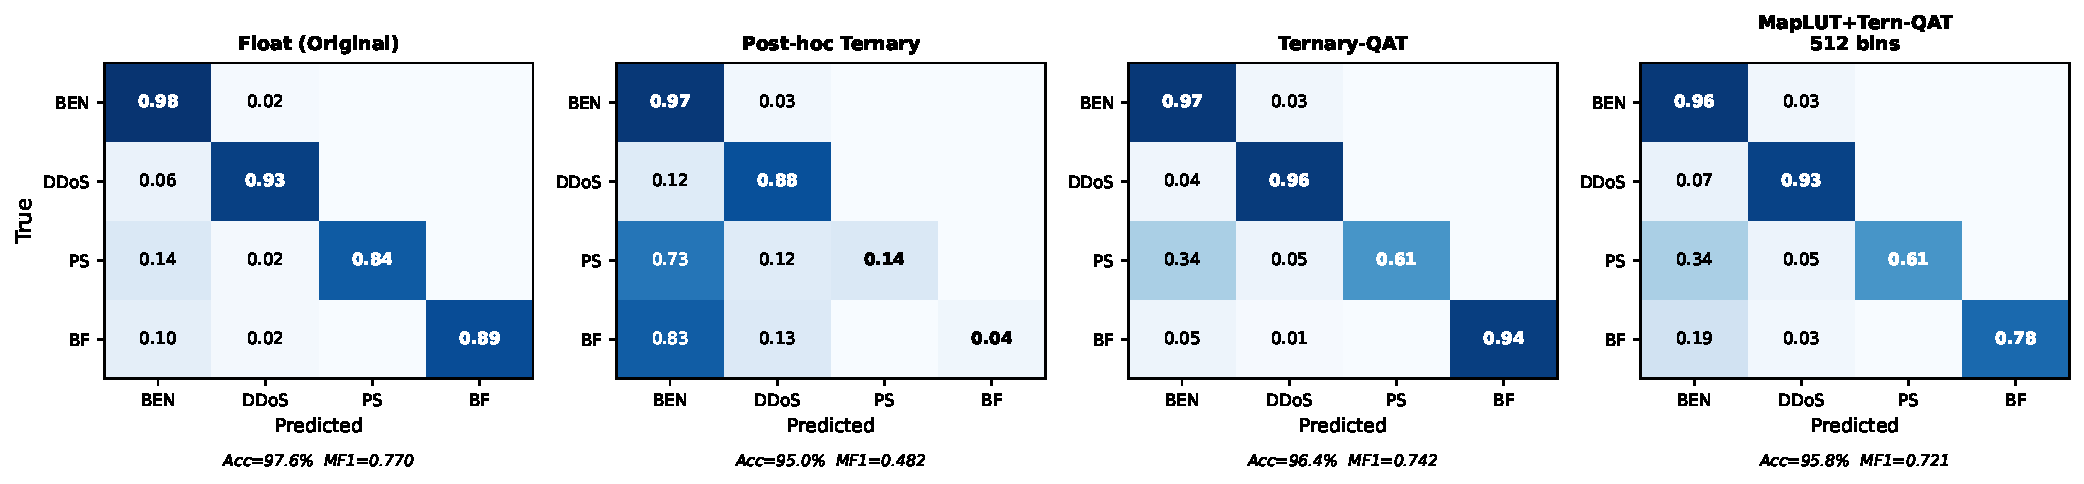
\includegraphics[width=\columnwidth]{figures/confusion_matrix.pdf}
\caption{Confusion matrices for four configurations.
Post-hoc ternary (upper right) collapses PortScan and BruteForce into
BENIGN.
Ternary-QAT (lower left) and MapLUT+Ternary-QAT 512b (lower right)
recover minority-class structure.}
\label{fig:confusion}
\end{figure}

\begin{figure}[t]
\centering
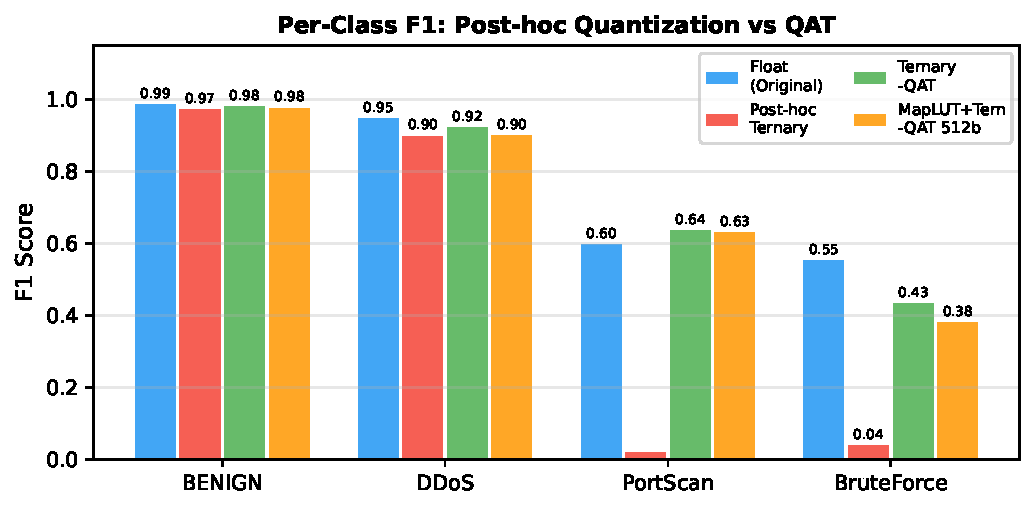
\includegraphics[width=\columnwidth]{figures/per_class_f1_comparison.pdf}
\caption{Per-class F1 comparison across configurations.
QAT-based methods (right two groups) recover minority classes;
PortScan~F1 under MapLUT+Ternary-QAT (0.629) exceeds the float baseline
(0.597).}
\label{fig:perclass}
\end{figure}

The per-class analysis (Figure~\ref{fig:perclass}) reveals the central
finding: post-hoc quantization primarily damages minority classes
(PortScan, BruteForce), while QAT-based methods maintain or improve
them.
BENIGN and DDoS classification remains strong ($\text{F1} > 0.93$)
across all configurations.
The PortScan F1 improvement from 0.597 to 0.629 under
MapLUT+Ternary-QAT is especially notable---it demonstrates that
\emph{aggressive quantization plus QAT can outperform float baselines
on hard classes}, because the training procedure forces representational
capacity toward difficult examples.

\subsection{Bins vs.\ Accuracy}\label{sec:bins}

The number of MapLUT bins $B$ controls the input-quantization
granularity.
Table~\ref{tab:bins} shows the trade-off for the MapLUT + Ternary-QAT
configuration using the QAT model.

\begin{table}[t]
\centering
\caption{MapLUT bin count vs.\ accuracy and memory
(MapLUT + Ternary-QAT, QAT model, $h{=}64$, 12 features).}
\label{tab:bins}
\small
\begin{tabular}{rcccr}
\toprule
Bins ($B$) & Accuracy & Macro F1 & PS F1 & LUT Memory \\
\midrule
64   & 82.55\% & 0.510 & 0.272 &  192\,KB \\
128  & 86.54\% & 0.618 & 0.540 &  384\,KB \\
256  & 91.97\% & 0.691 & 0.629 &  768\,KB \\
512  & 95.78\% & 0.721 & 0.629 & 1{,}536\,KB \\
\bottomrule
\end{tabular}
\end{table}

\begin{figure}[t]
\centering
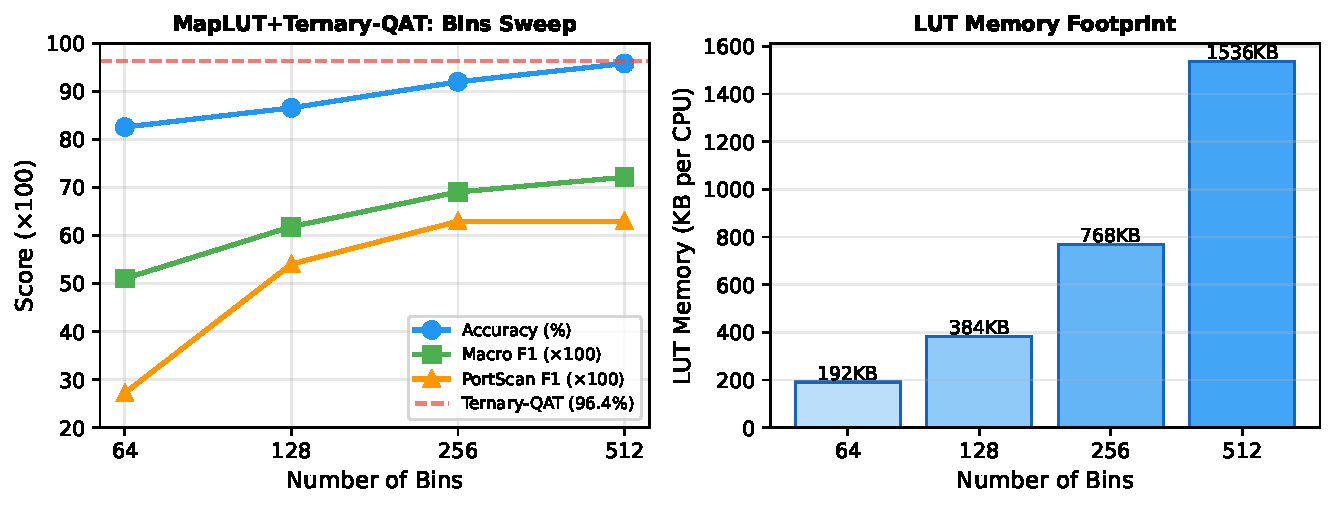
\includegraphics[width=\columnwidth]{figures/bins_sweep_qat.pdf}
\caption{Bins vs.\ accuracy and LUT memory for MapLUT + Ternary-QAT.
PortScan F1 saturates at 256 bins (0.629), while overall accuracy
continues to improve at 512 bins.}
\label{fig:bins}
\end{figure}

Accuracy improves monotonically with $B$ (Figure~\ref{fig:bins}).
PortScan F1 saturates at $B{=}256$ (0.629), suggesting that 256 bins
provide sufficient input resolution for minority-class discrimination.
Overall accuracy continues to improve from 91.97\% (256 bins) to
95.78\% (512 bins), primarily reflecting better BENIGN/DDoS separation
at finer granularity.
We select $B{=}512$ as the recommended configuration, achieving
95.78\% accuracy within 1.86~percentage points of the full int32
baseline while maintaining zero multiplications.

\subsection{Memory Analysis}\label{sec:memory}

Table~\ref{tab:memory} breaks down \sys's memory footprint for the
recommended 512-bin configuration.

\begin{table}[t]
\centering
\caption{\sys V3 memory layout ($B{=}512$, $h{=}64$).}
\label{tab:memory}
\small
\begin{tabular}{lr}
\toprule
Component & Size \\
\midrule
Model parameters (ternary + biases) & 1.8\,KB \\
MapLUT ($12 \times 512 \times 64 \times 4$\,B) & 1{,}536\,KB/CPU \\
Per-CPU scratch (\texttt{nn\_ctx}) & ${\sim}$300\,B/CPU \\
Flow map (65{,}536 entries) & ${\sim}$2\,MB shared \\
\bottomrule
\end{tabular}
\end{table}

The dominant cost is the MapLUT (1.5\,MB per CPU), which trades memory
for multiply-free computation.
On a 16-core server, the total LUT footprint is ${\sim}$24\,MB---well
within kernel memory budgets for modern servers with $>$32\,GB RAM.
The ternary model itself is remarkably compact at 1.8\,KB, a $3\times$
reduction over the int32 baseline's 5.6\,KB.
For memory-constrained deployments, the 256-bin configuration achieves
91.97\% accuracy at 768\,KB/CPU---a $2\times$ reduction with the same
PortScan~F1 of 0.629.


%% ============================================================
\section{Related Work}\label{sec:related}

\textbf{In-kernel ML via eBPF.}
Bachl~\etal~\cite{bachl2021dt} pioneered eBPF-based IDS with decision
trees on CIC-IDS-2017.
Hara~\etal~\cite{hara2023nn} demonstrated int8 NN inference in eBPF.
Zhang~\etal~\cite{zhang2024dsn} introduced the enlargement method with
tail-call chains.
Osaki~\etal~\cite{osaki2024} proposed dynamic fixed-point quantization.
Chen~\etal~\cite{chen2025kd} combined knowledge distillation with
decision trees.
All of these systems rely on multiply instructions;
\sys is the first to achieve zero-multiply inference.

\textbf{Multiply-free neural networks.}
AdderNet~\cite{chen2020addernet} replaces convolution multiplications
with $\ell_1$-distance, achieving competitive accuracy on ImageNet.
DeepShift~\cite{elhoushi2021deepshift} represents weights as powers of
two, converting multiplications to bit shifts.
ShiftAddNet~\cite{you2020shiftaddnet} combines shift and addition layers
in a hardware-inspired architecture.
LUT-NN~\cite{park2024lutnn} uses centroid learning with lookup tables
for efficient mobile inference.
These works target GPUs/ASICs with float support; \sys adapts
the LUT and ternary ideas to the unique constraints of eBPF's
integer-only, verifier-checked environment.

\textbf{Binary/ternary neural networks.}
XNOR-Net~\cite{rastegari2016xnor} binarizes both weights and
activations, replacing multiply-accumulate with XNOR + popcount.
TWN~\cite{li2016twn} introduced ternary weight networks with a
symmetric threshold.
\sys's TernaryShift builds on TWN but replaces the final scaling
multiplication with a bit shift calibrated to the ternary magnitude,
ensuring full compatibility with eBPF's instruction set.

\textbf{Quantization-aware training.}
Jacob~\etal~\cite{jacob2018quant} demonstrated that training with
simulated quantization in the forward pass and STE in the backward pass
yields integer-arithmetic-only models with minimal accuracy loss.
Bengio~\etal~\cite{bengio2013ste} provided the theoretical foundation
for straight-through estimators of discrete neurons.
\sys applies QAT to \emph{ternary} quantization in the context of
severely imbalanced security data, where we show that post-hoc
quantization fails catastrophically and QAT is essential.


%% ============================================================
\section{Conclusion}\label{sec:conclusion}

We presented \sys, the first eBPF/XDP neural inference engine with
zero multiply instructions.
Through operator co-design---MapLUT for the input layer and TernaryShift
for hidden layers---and quantization-aware training with straight-through
estimation, \sys achieves 95.78\% accuracy on CIC-IDS-2017 with 1,424
BPF instructions, none of which are multiplications.
The QAT procedure is critical: post-hoc ternary quantization
catastrophically collapses minority-class performance (PortScan F1
drops to 0.020), while QAT with focal loss not only recovers but
\emph{improves} PortScan F1 to 0.629, exceeding the float baseline's
0.597.

\textbf{Limitations.}
The accuracy gap between zero-multiply (95.78\%) and full int32 (97.64\%)
is non-trivial.
The 512-bin LUT requires 1.5\,MB per CPU, which may be prohibitive on
resource-constrained embedded devices.
EarlyExit in its current form hurts accuracy (74.88\%) and is not
recommended for deployment.

\textbf{Future work} includes:
(1)~improving EarlyExit with class-aware confidence thresholds to safely
skip easy traffic;
(2)~live XDP deployment with \texttt{tcpreplay} to measure end-to-end
throughput;
(3)~online model retraining with hot LUT updates for concept-drift
adaptation; and
(4)~extending QAT to binary (1-bit) weights for further compression.


%% ============================================================
\bibliographystyle{ACM-Reference-Format}
\bibliography{references}

\end{document}
